\documentclass[a4paper,twoside]{article}

\usepackage{epsfig}
\usepackage{times}
\usepackage{subcaption}
\usepackage{calc}
\usepackage{amstext}
\usepackage{amsthm}
\usepackage{multicol}
\usepackage{pslatex}
\usepackage{apalike}
\usepackage[ruled,vlined,caption2]{algorithm2e}
\usepackage[bottom]{footmisc}
\usepackage{SCITEPRESS} 
\usepackage{cite}
\usepackage{amsmath,amssymb,amsfonts}
\usepackage{graphicx}
\usepackage{textcomp}
\usepackage{xcolor}
\usepackage{amsmath}
\usepackage{tabularx}
\usepackage{adjustbox}
\usepackage{titlesec}
\usepackage{pgfplots}
\usepackage{pgf-pie}
\usepackage{csvsimple}
\usepackage{booktabs}
\usepackage{float}

\begin{document}

% Define title font
\titleformat{\title}{\fontsize{15pt}{18pt}\bfseries}{\thetitle}{1em}{}
\title{Addressing Educational Disparities: Assessing the Gap for Indigenous Community}

\author{\authorname{Dr. Shafaq Khan, Viutika Rathod, Abhirup Ranjan, Anika Anjum Una and Neel Manish Pandya}
\affiliation{School of Computer Science,University of Windsor, Ontario,Canada}
}

\keywords{Indigenous Knowledge, Indigenous Perspectives, Educational Disparities, Indigenous Students, NoSQL-MongoDB Database}

\abstract{This research paper explores the integration of Indigenous knowledge and perspectives in education to address the educational disparities faced by Indigenous students in Canada \cite{Change23}. It proposes a management system utilizing a NoSQL-MongoDB database and logistic regression model to predict student dropout rates based on key factors such as Cultural Identity, Gender, Government Funding, and more \cite{GovtOfCanada21}. The logistic regression model achieved an accuracy rate of 0.831 on the testing dataset and provided valuable insights into the factors influencing dropout rates among Indigenous students. The paper emphasizes the importance of cultural sensitivity, ethical considerations, and collaboration with Indigenous communities throughout the research process. While logistic regression offers interpretability and simplicity, future work may explore the use of other machine learning models and qualitative data to enhance accuracy and gain deeper insights. The goal is to promote educational equity and inclusivity while respecting Indigenous knowledge and aspirations in Canadian education.}

\onecolumn \maketitle \normalsize \setcounter{footnote}{0} \vfill

\section{\uppercase{Introduction}}
\label{sec:introduction}

The Indigenous communities in Canada experience significantly higher dropout rates compared to non-Indigenous communities in this part of the world, attributed to a range of factors such as historical and inter-generational impacts, financial inequities, social marginalization, lack of support systems, and geographic barriers \cite{GovtOfOntario17}. These factors restrict access to quality education for Indigenous students, resulting in lower educational achievements compared to the general population of Canada \cite{CFSOntario21}.\\Outline of the problem of educational disparities faced by Indigenous students in Canada, there are multiple factors such as the legacy of colonialism, residential schools, racism, and insufficient funding hinder access to post-secondary education, which is recognized as a treaty right for Indigenous students. Funding inadequacy and access difficulties contribute to a significant disparity in educational opportunities \cite{Brown23}. Also, the lack of necessary infrastructure has hindered the distribution of culturally relevant educational curricula to Indigenous communities. Teaching practices in non-Indigenous institutions need refinement, focusing on incorporating Indigenous history, cultures, and perspectives, and addressing racism and
marginalization \cite{GovtOfCanadaEthics19}.\\Our work in this research paper is motivated by a deep understanding of past injustices and current hardships faced by Indigenous communities. We aim to address the lack of cultural responsiveness in the mainstream educational system and promote justice, fairness, and reconciliation \cite{Weston19}. By embracing empathy and recognizing the generational effects of policies like the residential school system, we seek to restore pride, dignity, and self-respect among Indigenous children \cite{Kim19}. Through cultural responsiveness, we aim to foster respect, understanding, and inclusive education for all students.\\Our objective here is to bridge the educational gap between Indigenous and non-Indigenous populations in Canada by addressing issues such as insufficient funding, cultural disconnection, discrimination, and lack of support systems for Indigenous communities. We aim to assess and analyze the quality of education for Indigenous students, promote evidence-based decision making, and ensure educational equity. Integrating Indigenous knowledge systems, languages, and histories into the curriculum is a crucial focus, empowering
Indigenous students and improving the educational experience for all.
\\To achieve our goals, we propose a model that utilizes a NoSQL database
i.e. MongoDB, to address educational disparities faced by Indigenous students.
Also using the Logistic Model we will capture unique information such
as cultural identity, language proficiency, community involvement, gender,
and other relevant details, while adhering to Indigenous data governance
principles. This will assist us in determining whether a particular person
may drop out, and if so, it will enable concerned local or governmental
bodies to take appropriate action. It will also enable comprehensive data
integration from various sources, evaluating the success of educational initiatives and facilitating timely support and prevention of widening educational gaps. The chosen NoSQL database ensures data privacy and security, aligning with ethical principles and relevant laws. There is a lack of published papers addressing our identified issue, making our research work unique. Through our comprehensive model and data-driven approach, we aim to contribute to the development of effective strategies and policies that empower Indigenous students and bridge the educational gap in Canada.

\section{\uppercase{Background Study}}
\label{sec:Literature Review}
This paper explores the role of educators, particularly those teaching aspiring conservation practitioners, in responding to the Truth and Reconciliation Commission (TRC) and the National Inquiry into Missing and Murdered Indigenous Women and Girls (MMIWG). The emphasis is on the significance of reconciliation and ethical engagement with Indigenous Peoples through a revolutionary approach to teaching indigenous knowledge. The focus is on fostering understanding, empathy, and respect for Indigenous knowledge and aspirations while equipping students with critical analysis skills for ethical engagement. The paper calls for universities to "Indigenize" their approaches, embracing anti-racism, humility, reciprocity, and confronting ongoing colonialism and white supremacy. The goal is to create a learning environment that respects and values Indigenous scholars, knowledge,and voices, fostering re-conciliatory relationships between conservation practitioners and Indigenous Peoples. Efforts should go beyond course content and focus on building an anti-racist, anti-oppressive campus culture that
centers Indigenous perspectives and enables Indigenous intellectual expression. The paper advocates for hiring more Indigenous faculty members and centering Indigenous Peoples as experts about themselves in the curriculum. The goal is to prepare students to engage with Indigenous Peoples in a just and affirming manner while respecting Indigenous knowledge and aspirations. The possible difficulties of successfully integrating Indigenous knowledge within the current curriculum and ensuring cultural sensitivity and authenticity in its application might, 
 however, be a drawback of this strategy \cite{Wu19}.
\\This paper focuses on the use of digital technologies to support Indigenous people’s language and literacy learning, particularly in English. Here, the emphasis is on addressing the negative inter-generational impacts of colonization and socioeconomic stress on Indigenous academic performance. The systematic review of 25 empirical studies provides insights into the efficacy of digital technology in supporting Indigenous learners. While the studies demonstrate positive outcomes, there are limitations, such as the lack of rigorous research methods and comprehensive reporting. To improve the effectiveness
of digital technology-based interventions, future research should
consider culturally relevant multiliteracies frameworks, engage in longitudinal studies to track students’ progress and incorporate more Indigenous cultural elements. Additionally, there is a need for data coding schemes to capture the nuances of Indigenous language and literacy learning. The research emphasizes the importance of culturally responsive practices, partnership with Indigenous communities, and addressing the unique contextual factors affecting Indigenous education. The reliance on digital infrastructure and access to technology, however, may be a weakness of their strategy or approach and present difficulties in isolated or disadvantaged Indigenous communities where dependable internet connectivity may be scarce \cite{JiaLi21}.
\\This paper presents the NOW (Northern Oral Language and Writing) Play project aiming to support young
children’s oral language and writing skills in northern rural and Indigenous communities. The research emerged from the concerns raised by kindergarten teachers in northern Canadian communities about students’ limited language abilities upon entering school. The project involved collaborating with public school divisions in small rural communities and local education authorities in Indigenous regions of four Canadian provinces. Focusing on the assessment and support of young children’s oral language and writing development in play contexts. These communities face challenges related to geographic isolation, limited teaching resources, and a lack of opportunities for teachers’ professional learning. The project emphasized the use of play contexts to enhance children’s language and literacy skills. Additionally, the project aimed to develop a culturally relevant oral language assessment tool. This tool was designed to capture the diverse ways in which children use language for various social purposes during play and small-group academic
activities. Teachers and researchers collaboratively analyzed video
recordings and transcripts of children’s play to identify different language uses and track individual children’s language development \cite{Stagg16}. However, the project also acknowledges challenges such as parental resistance to play based approaches and the necessity for cultural sensitivity in research methods. Careful navigation of these obstacles is crucial to ensure the project’s ultimate success and positive impact.
\\All these studies focus on the integration of indigenous knowledge across
a range of educational contexts. These papers acknowledge the challenges
and limitations in implementing the overall goal of integrating Indigenous
knowledge and perspectives in education.

\section{\uppercase{Proposed Model}}
\label{sec:Proposed Methodology}
In this section, we propose a predictive model using Logistic Regression, a
binary classification algorithm. The model predicts whether a student will
drop out (1) or not (0) by using the key factors that have been identified
as input variables. Its interpretable results allow for a clear understanding of the impact of predictor variables on dropout rates, helping to identify key factors contributing to the disparities \cite{Das21}. Moreover, logistic regression provides probability estimates, prioritizing higher-risk students for support systems. With its low complexity, minimal data preprocessing requirements, and ease of implementation, logistic regression offers a practical and efficient solution for handling the data management system. While it may not capture complex relationships as effectively as advanced algorithms, combining it with other techniques through ensembling could further enhance its predictive performance and lead to more comprehensive strategies for bridging the educational gap among Indigenous communities.

The proposed model takes a systematic approach to predicting the likelihood of dropout among Indigenous students (as shown in Figure~\ref{fig:flowdiagram}). It starts by compiling pertinent
data from various sources, such as governmental agencies and academic
institutions \cite{Bisong19}. 
\begin{figure}[H]
    \centering 
    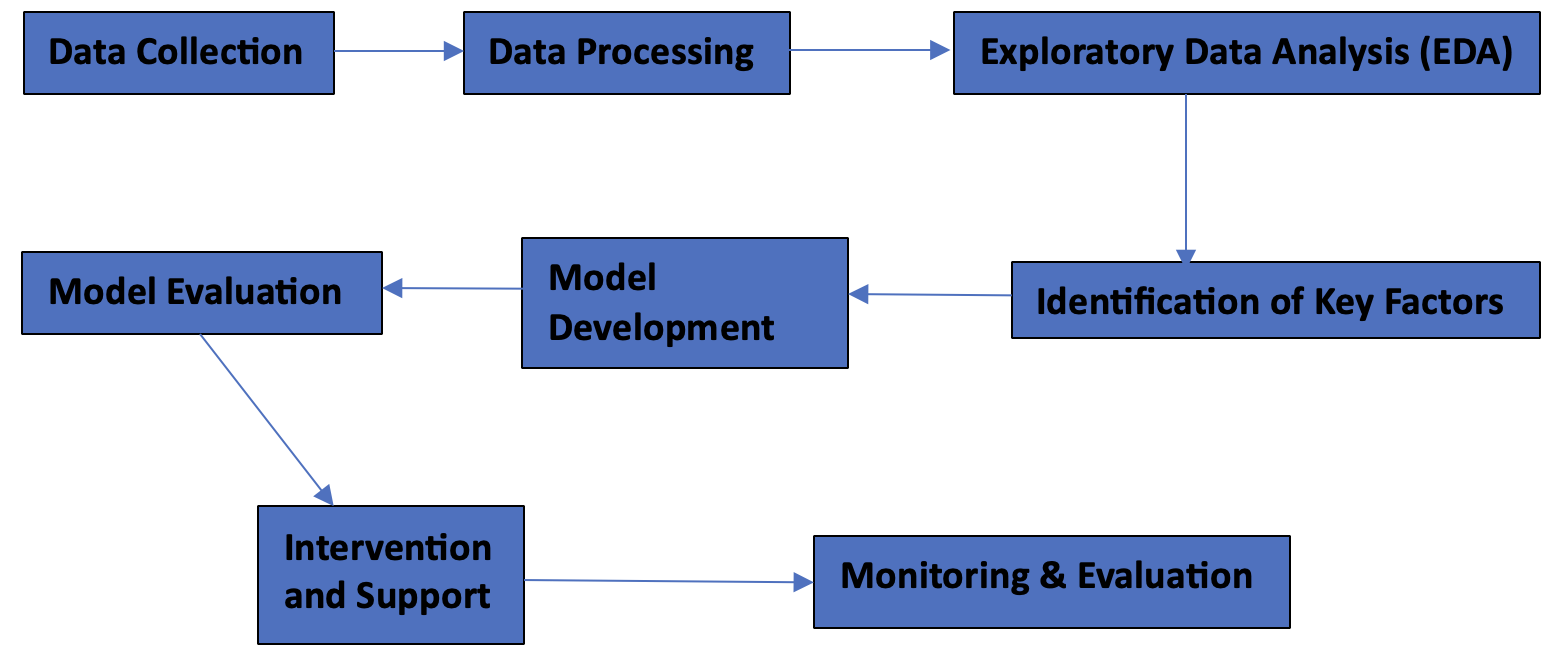
\includegraphics[width=0.5\textwidth, angle=0]{images/FlowDiagram.png}	
    \captionsetup{format=plain, justification=centering}
    \caption{Workflow diagram.}
    \label{fig:flowdiagram}
\end{figure}

Key traits like cultural identity, language proficiency, and educational level are chosen after the data has been preprocessed. Following that, the dataset is divided into training and test sets. To determine the correlation between the selected features and dropout outcomes, the logistic regression model is trained using the training data. The model is tested on the testing set, and metrics like accuracy, precision, recall, F1-score, and ROC-AUC \cite{GMK20} are used to assess its performance. An effective predictive model for comprehending dropout patterns among Indigenous students is being developed through this thorough process.

\section{\uppercase{Methodology and Experimentation}}
\label{sec:Results}
The logistic regression model was implemented as part of our proposed management system to address educational disparities faced by Indigenous students in Canada. The model's objective was to predict the likelihood of student dropout (1) or non-dropout (0) based on key factors, including Cultural Identity, Gender, Government Funding, Type of Educational Institute, Employment Sector, Language Proficiency, Community Involvement, Age, and Level of Education. We trained the model using a binary classification algorithm and evaluated its performance using various metrics.

\subsection{Data Collection}

A variety of sources, including the Alberta Open Data Portal, Statistics Canada, the FNIGC (First Nations Information Governance Center), and the Government of British Columbia, were used to collect the data for data preprocessing in Indigenous education research. The dataset comprises diverse information, including demographic data, cultural identity, gender, government funding, enrollment figures, and academic performance metrics. To ensure accuracy and suitability for analysis, the data underwent rigorous cleaning, transformation, and organization processes. Outliers were addressed, features were normalized or encoded as required, and missing values were imputed. Such preprocessing is crucial for subsequent analysis, such as logistic regression modeling, which aims to shed light on the variables influencing the academic performance and dropout rates of Indigenous students.


The Figure~\ref{fig:datacollection} illustrates the credential they have achieved so far in the Alberta region based on the dataset available on Alberta Open Data Portal website.
 \begin{figure}[H]
    \centering 
    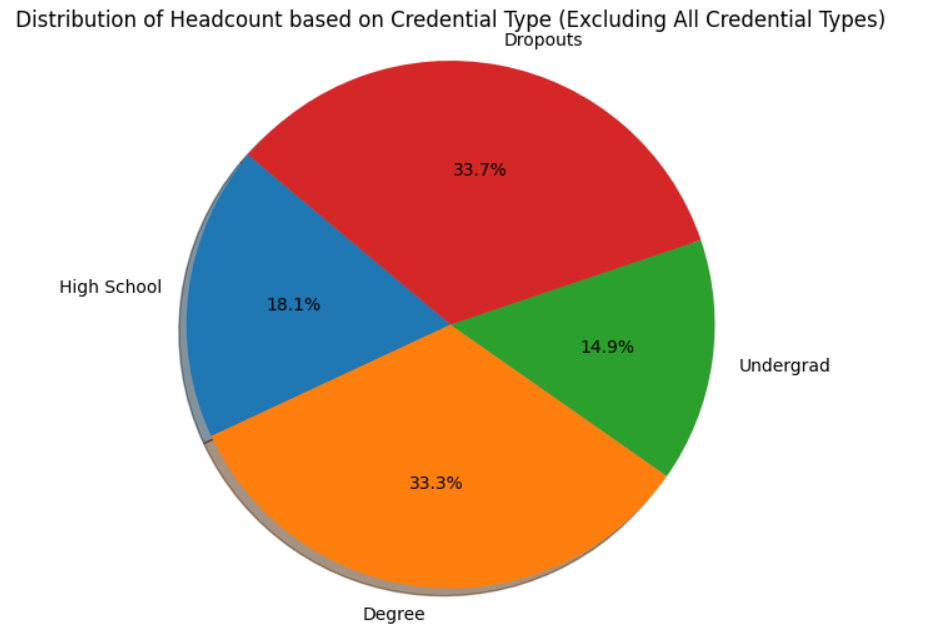
\includegraphics[width=0.5\textwidth, angle=0]{images/DataCollection.png}	
    \captionsetup{format=plain, justification=centering}
    \caption{Distribution of Indigenous students based on their education level in Alberta Region.}
    \label{fig:datacollection}
\end{figure}




\subsection{Data Processing}
For data preprocessing, we will be categorizing the fields into two categories:
Binary and Numerical variables \cite{Mallikharjuna23}. After one-hot encoding, there will be
only two values for categorical variables which we will include as binary
variables. Here is the categorization:
\\
\\
\textbf{Binary Variables}

\begin{itemize}
    \item \textbf{Cultural Identity (after binary encoding)}
    \begin{itemize}
        \item First Nations (1 for "First Nations", 0 for others)
        \item Inuit (1 for "Inuit", 0 for others)
        \item Métis (1 for "Métis", 0 for others)
    \end{itemize}

    \item \textbf{Gender (after binary encoding)}
    \begin{itemize}
        \item Gender (1 for "Female", 0 for "Male")
    \end{itemize}

    \item \textbf{Government Funding (after binary encoding)}
    \begin{itemize}
        \item Government Funding (1 for "Yes", 0 for "No")
    \end{itemize}
\end{itemize}

\textbf{Numerical Variables}

\begin{itemize}
    \item \textbf{Language Proficiency (after label encoding)}
    \begin{itemize}
        \item Language Proficiency (0 for "Basic", 1 for "Intermediate", 2 for "Advanced")
    \end{itemize}
    
    \item \textbf{Community Involvement (after label encoding)}
    \begin{itemize}
        \item Community Involvement (0 for "Low", 1 for "Medium", 2 for "High")
    \end{itemize}
    
    \item \textbf{Age (Numerical variable)}
    \begin{itemize}
        \item Age (numeric values)
    \end{itemize}
    
    \item \textbf{Level of Education (after label encoding)}
    \begin{itemize}
        \item Level of Education (0 for "School", 1 for "High School", 2 for "Bachelor’s", 3 for "Master’s", etc.)
    \end{itemize}
    
    \item \textbf{Type of Educational Institute (after label encoding)}
    \begin{itemize}
        \item Type of Educational Institute (0 for "Public School", 1 for "Private School", 2 for "Homeschooling", 3 for "Online Learning")
    \end{itemize}
    
    \item \textbf{Employment Sector (after label encoding)}
    \begin{itemize}
        \item Employment Sector (0 for "Government", 1 for "Private", 2 for "Others")
    \end{itemize}
\end{itemize}

\begin{table}[htbp]
    \caption{Summary of Categorical and Numerical Features in the Dataset.}
    \label{tab:example2}
    \small % Set the font size to 9pt
    \begin{tabularx}{\columnwidth}{|X|X|}
        \hline
        {Field} & {Category} \\
        \hline
        First Nations & Binary (Cultural Identity) \\
        \hline
        Inuit & Binary (Cultural Identity) \\
        \hline
        Métis & Binary (Cultural Identity) \\
        \hline
        Gender & Binary \\
        \hline
        Government Funding & Binary \\
        \hline
        Language Proficiency & Numerical (Ordinal) \\
        \hline
        Community Involvement & Numerical (Ordinal) \\
        \hline
        Age & Numerical (Ordinal) \\
        \hline
        Level Of Education & Numerical (Ordinal) \\
        \hline
        Type of Educational Institute & Numerical (Ordinal) \\
        \hline
        Employment Sector & Numerical (Ordinal) \\
        \hline
    \end{tabularx}
\end{table}


\subsection{Feature Selection}
Recursive feature elimination (RFE) \cite{Mishra20} is used in the proposed algorithm
for addressing educational disparities among Indigenous students in Canada
to pinpoint the key characteristics that significantly influence the likelihood of dropout prediction made by logistic regression. Initially, the logistic regression model is trained using all pertinent features, including binary and numerical variables. Following a systematic elimination of less significant features, the RFE process ranks the remaining features according to how well they predict academic outcomes. The subset of crucial elements with the greatest influence on Indigenous students’ dropout rates is identified through this iterative process.

\begin{algorithm}
    \SetAlgoNlRelativeSize{0}
    \SetAlgoNlRelativeSize{-1}
    \KwData{Input data $X$, Target variable $y$}
    \KwResult{Selected features $X_{\text{selected}}$}
    
    Encode categorical features\;
    $X_{\text{enc}} \gets \text{OneHotEncode}(X)$\;
    
    Split data into training and testing sets\;
    $X_{\text{train}}, X_{\text{test}}, y_{\text{train}}, y_{\text{test}} \gets \text{split}(X_{\text{enc}}, y, \text{test\_size} = 0.2, \text{random\_state} = 42, \text{stratify} = y)$\;
    
    Create logistic regression model with balanced class weights\;
    $model \gets \text{LogisticRegression}(\text{class\_weight} = \text{'balanced'})$\;
    
    Implement RFE for feature selection\;
    $\text{num\_features} \gets 5$\;
    $rfe \gets \text{RFE}(model, \text{n\_features\_to\_select} = \text{num\_features})$\;
    $rfe.\text{fit}(X_{\text{train}}, y_{\text{train}})$\;
    
    Fit model on selected features\;
    $X_{\text{train\_sel}} \gets X_{\text{train}}[:, rfe.\text{support\_}]$\;
    $model.\text{fit}(X_{\text{train\_sel}}, y_{\text{train}})$\;
    
    Predict target variable on the testing set\;
    $X_{\text{test\_sel}} \gets X_{\text{test}}[:, rfe.\text{support\_}]$\;
    $y_{\text{pred}} \gets model.\text{predict}(X_{\text{test\_sel}})$\;
    
    Calculate F1-score and accuracy\;
    $f1 \gets \text{F1-score}(y_{\text{test}}, y_{\text{pred}})$\;
    $accuracy \gets \text{accuracy\_score}(y_{\text{test}}, y_{\text{pred}})$\;
    
    Print results\;
    \textbf{print}("F1-score for 'Dropout':", f1)\;
    \textbf{print}("Accuracy:", accuracy)\;

    \caption{Algorithm: Feature Selection using RFE and Logistic Regression.}
\end{algorithm}

The F1-score is used in the above algorithm to evaluate how well the
logistic regression model predicted educational outcomes for Indigenous students. Particularly when working with datasets that are unbalanced, it aids in assessing the model’s capacity to balance precision and recall. The computational complexity of RFE, which is roughly O($np^2/2$), is also taken into account when choosing the features. With RFE’s iterative design, subsets of features are used to train the logistic regression model, allowing for the effective identification of key predictors to reduce educational disparities among Indigenous communities.


\subsection{Data Split}
The "train-test split," in which the dataset is divided into two parts: “\textbf{a training set}” and  “\textbf{a test set}”, is the most popular data splitting technique.
\begin{enumerate}
  \item The training set and the test set should be separated from the dataset. The logistic regression model will be trained using the training set, and its performance will be assessed using the test set
  \item The split ratio is typically 80\% training data and 20\% test data, but it can be changed depending on the size of the dataset and the particular requirements.
\end{enumerate}

\subsection{Model Training}

In order to accurately predict whether a student is likely to drop out (1) or not (0) based on the selected features: "Cultural Identity," "Gender," "Government Funding," "Type of Educational Institute," "Employment Sector," "Language Proficiency," "Community Involvement," "Age," and "Level of Education," the logistic regression model must be trained to recognize patterns and relationships within the training data \cite{Parker13}.

For each data point in the training set, the calculated values in the context of logistic regression refer to the linear combinations of the chosen features ('Cultural Identity', 'Gender', 'Government Funding', 'Type of Educational Institute', 'Employment Sector', 'Language Proficiency', 'Community Involvement', 'Age', 'Level of Education'). For each data point, the model will compute a weighted sum of the feature values and add a bias term. The linear combination (y) for a single data point (x) is computed mathematically as follows:
\begin{align}
y &= b_0 + b_1 x_1 + b_2 x_2 + \ldots + b_n x_n
\end{align}

\textbf{Here:}
\begin{itemize}
  \item y is the calculated value for a given data point.
  \item b0 is the bias term (intercept).
  \item b1, b2, ..., bn are the weights (coefficients) assigned to each feature.
  \item x1, x2, ..., xn are the feature values for the corresponding data point.
\end{itemize}

The calculated values (y) will then be subjected to the sigmoid function to convert them into probabilities. The formula for the function is:
\begin{align}
p &= \frac{1}{1 + \exp(-y)}
\end{align}

\begin{figure}[H]
    \centering 
    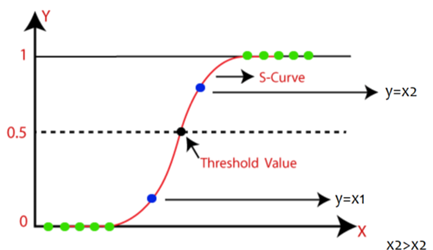
\includegraphics[width=0.5\textwidth, angle=0]{images/SGraph.png}	
    \captionsetup{format=plain, justification=centering}
    \caption{The S Curve: Visualization of Logistic Regression's Probabilistic Model.}
    \label{fig:fig_mom0}
\end{figure}

Thus, p is the logistic regression model's output—the likelihood that a student will drop out—for a specific data point.\\
The exponential representation of -y is represented by ${exp^{-y}}$.
No matter the range of the calculated values (y), the sigmoid function (as shown in Figure~\ref{fig_mom0} \cite{Essampally20}) will make sure that the output probabilities (p) are bounded between 0 and 1. For the corresponding data point, the model will predict a dropout (1) when p is greater than or equal to 0.5, and a non-dropout (0) when p is less than or equal to 0.5.
The regression algorithm will iteratively adjust the weights (b1, b2,..., bn) and the bias term (b0) during the model training process using optimization techniques like gradient descent. The goal is to identify the best combination of weights and biases to minimize the discrepancy between the predicted probabilities and the actual binary outcomes (dropout or non-dropout) in the training data, thereby enhancing the model's capacity to make precise predictions on fresh, untested data.

\subsection{Model Evaluation}
Evaluation metrics like accuracy, precision, recall, F1-score, and ROC-AUC (Area Under the Curve - Receiver Operating Characteristic) are used to assess the performance of the logistic regression model, which was trained using the features like Cultural Identity, Gender, Government Funding, Type of Educational Institute, Employment Sector, Language Proficiency, Community Involvement, Age, and Level of Education. These metrics evaluate how well the model performs in accurately predicting Indigenous students' likelihood of dropping out of school. We can assess the model's efficacy in addressing educational disparities and promoting educational equity among Indigenous communities in Canada by analyzing these evaluation results on the testing dataset.

\subsection{Interpretability}
The logistic regression model's feature importance (coefficients) offers important insights into how each feature affects the likelihood that Indigenous students will drop out of school. While negative coefficients suggest factors linked to lower dropout rates, positive coefficients point to factors linked to higher dropout rates. Stakeholders can pinpoint key causes of educational disparities by looking at these coefficients for categories like Cultural Identity, Gender, Government Funding, Type of Educational Institute, Employment Sector, Language Proficiency, Community Involvement, Age, and Level of Education. In order to promote educational equity for Indigenous communities, targeted interventions and support systems are informed by this understanding. While there are other interpretability techniques, Feature Importance (Coefficients) stands out for its clarity, usability, and universal interpretability, enabling evidence-based decision-making to effectively close the educational gap for Indigenous students.

\section{\uppercase{Results}}
The logistic regression model demonstrated promising results in predicting dropout rates among Indigenous students. The model achieved an accuracy rate of 0.831 on the testing dataset, indicating its ability to correctly classify dropout outcomes. Moreover, the F1 score was 0.831 (as shown in Figure~\ref{fig:result}), showcasing its effectiveness in identifying students at risk of dropping out and minimizing false positives.

The interpretability of the logistic regression model allowed us to identify key factors influencing dropout rates among Indigenous students. The coefficients for various features provided valuable insights into the impact of Cultural Identity, Gender, Government Funding, Type of Educational Institute, Employment Sector, Language Proficiency, Community Involvement, Age, and Level of Education on educational outcomes. For instance, positive coefficients indicated factors associated with higher dropout rates, while negative coefficients pointed to factors linked to lower dropout rates. This understanding empowered us to design targeted interventions and support systems to enhance educational equity and bridge the educational gap for Indigenous students in Canada.


\begin{figure}[!htb]
	\centering 
	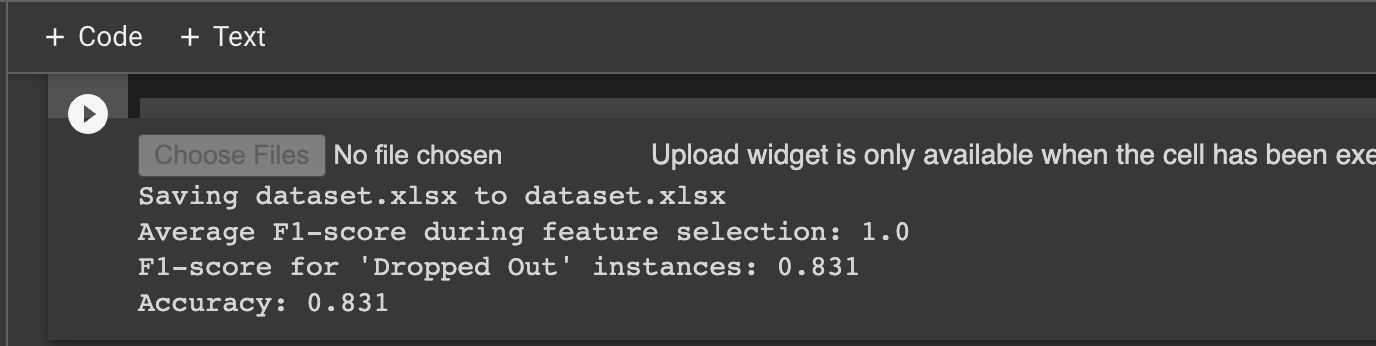
\includegraphics[width=1.0\linewidth,keepaspectratio]{images/Result.png}
        \captionsetup{format=plain, justification=centering}
	\caption{Showing the Accuracy for Dropped out instances for Indigenous Students.} 
	\label{fig:result}
\end{figure}


\section{\uppercase{Limitations/Challenges}}
While the proposed approach to address educational disparities faced by Indigenous students in Canada through the utilization of a NoSQL database (MongoDB) and logistic regression model is promising, there are a few limitations that must be considered.

Initially, our approach was highly data-driven and relied on the quantity and availability of data. The indigenous communities we are working on along with their historical factors, privacy concerns, and limited data collection impose challenges in obtaining correct and descriptive data. Missing values in features or target variables can lead to biased estimates and inaccurate predictions, even with imputation techniques, which may introduce biases of their own. Additionally, biased data with over/underrepresented groups can result in unfair and discriminatory predictions, requiring proactive measures to address data bias. Outliers, as extreme values, can exert undue influence on model parameters and should be properly detected and handled for improved accuracy. Moreover, sampling bias arising from non-random or unrepresentative data collection can hinder model generalization to new data. Data heterogeneity stemming from diverse sources may necessitate harmonization efforts to ensure meaningful analysis.

Canada's Indigenous communities encompass a rich tapestry of diversity, comprising over 600 recognized First Nations, Métis, and Inuit communities, each with distinct cultural and socio-economic backgrounds. Acknowledging and comprehending these complexities are essential in addressing the educational disparities faced by Indigenous students. Cultural diversity plays a pivotal role as communities may prioritize traditional knowledge and language preservation, while others seek to integrate modern education with their heritage. Socioeconomic factors add another layer of variation, with economic realities varying between remote communities, where opportunities may be limited, and urban populations facing unique challenges that influence educational access and outcomes. Historical traumas, like colonization, continue to impact educational engagement and demonstrate resilience in preserving their cultures. Language and identity are intertwined and directly influence educational experiences. Moreover, access to educational resources differs across communities. Disparities also diverge between remote and urban Indigenous communities, driven by geographic barriers and infrastructure challenges.

Addressing resource constraints requires strategies and collaborative efforts. Limited funding poses challenges for educational initiatives, data management systems, and advanced analytics, alongside the high costs of technology infrastructure and skilled personnel. Moreover, technical constraints like the lack of specialized expertise, unreliable internet connectivity in remote communities, and resistance to technological changes add complexity.

In addition, our model, logistic regression, may provide insights into factors contributing to dropout rates, but it might not capture all the complexities of the educational disparities faced by Indigenous students. The model assumes linear relationships, but educational disparities may involve non-linear, interactive, or complex patterns that it may not capture effectively. One major drawback is its limited ability to capture nonlinear decision boundaries, which may not adequately represent situations influenced by multiple factors. Additionally, it might overlook important feature interactions, like cultural identity or community involvement, leading to oversimplified predictions. Handling high-dimensional data can be challenging due to issues like multicollinearity and overfitting. Its reliance on numeric features also makes it difficult to handle non-numeric data, such as categorical or textual variables, without increasing model complexity. Moreover, there exists a trade-off between model interpretability and predictive accuracy, with logistic regression being interpretable but potentially sacrificing performance in complex educational scenarios.

In addressing educational disparities, incorporating other machine learning models such as SVM, decision trees, clustering, and statistical techniques like correlation analysis and multiple regression analysis can offer a more comprehensive understanding of the complexities involved and enhance predictive accuracy based on dataset characteristics and research goals.
In conducting research in Indigenous education, upholding ethical principles is paramount. This includes obtaining informed consent and safeguarding sensitive data to protect confidentiality, while also respecting Indigenous values and involving communities in decision-making processes. Researchers must be cautious not to perpetuate stereotypes or stigmatize communities and demonstrate cultural sensitivity by acknowledging traditions and historical context. Transparency and accountability are essential, in documenting methodology and sharing findings with communities. The focus should be on benefiting Indigenous communities, aligning research outcomes with their goals, and ensuring the long-term sustainability of data systems. Empowering Indigenous voices and addressing power imbalances in research is vital for promoting inclusivity and driving positive change in Indigenous education \cite{Chiddi19}. 

\section{\uppercase{Conclusion and Future Work}}
The future work of this research paper holds promising directions to enhance its impact and tackle additional challenges in Indigenous education. Ensuring data privacy and security while collaborating with Indigenous communities is essential for comprehensive data collection. Cultural sensitivity should be prioritized throughout the research process to respect community values and align research outcomes with their needs. Incorporating qualitative data alongside quantitative measures can provide deeper insights into Indigenous students' experiences. Exploring various machine learning models and forming collaborations between academic institutions, government agencies, and Indigenous communities can lead to more accurate predictions and sustainable change. Ultimately, future research should focus on promoting equitable and inclusive education while addressing educational disparities faced by Indigenous students. In conclusion, the logistic regression model proved to be a valuable tool in addressing educational disparities faced by Indigenous students. Its accuracy and interpretability allowed for the identification of significant predictors of dropout, enabling the development of evidence-based strategies for educational improvement. By incorporating Indigenous data governance principles and utilizing MongoDB as a NoSQL database, our management system offers a unique and comprehensive solution to empower Indigenous communities and promote educational equity in Canada. The integration of Indigenous knowledge systems, languages, and histories into the curriculum further enhances the educational experience for all students and fosters reconciliation. With our research and data-driven approach, we aim to contribute to the development of effective policies and strategies that promote justice, fairness, and inclusivity in education for Indigenous communities.

\newpage
\bibliographystyle{apalike}
{\small
\bibliography{references}}





\end{document}

